\documentclass[fontsize=12pt]{article}
\usepackage[utf8]{inputenc}

% AMS Math


\usepackage[a4paper, total={6in, 8in}]{geometry}
\usepackage{amsmath}
\usepackage{amsfonts}
\usepackage{amssymb}
\usepackage{natbib}
\usepackage{graphicx}
\usepackage{url}
\usepackage{hyperref}
\usepackage{xcolor}

\newcommand{\calM}{\mathcal{M}}

\title{Convergence of Geodesic and Euclidean distances on an Embedded Riemannian Manifold}
\author{
	Kisung You\\
	\texttt{kyoustat@gmail.com}
}

\date{\today}



\begin{document}

\maketitle

\section{Introduction}

Let $(\calM,g)$ be a complete Riemannian manifold of dimension $m$ embedded in $\mathbb{R}^n$. One conventional example is a 2-dimensional hypersphere $\mathbb{S}^2$ in 3-dimensional Euclidean space, as in Figure \ref{fig:sphere}. For $A, B \in \mathbb{S}^2$, an easy way to connect two points would be a {\color{red}\bf straight line} in $\mathbb{R}^3$. However, if the domain is restricted to $\mathbb{S}^2$ (surface of the sphere), {\color{blue}\bf geodesic} is the shortest path while preserving geometry of the underlying manifold.


\begin{figure}[htbp]
	\centering
	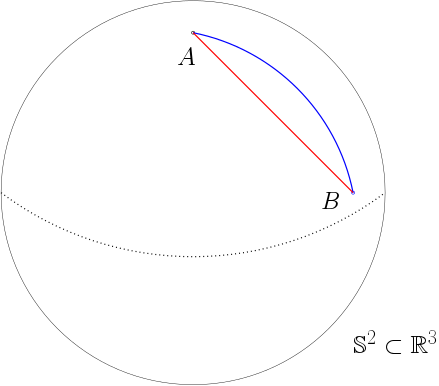
\includegraphics[width=0.55\linewidth]{figure_twodist.png}
	\caption{connecting two points $A, B \in \calM = \mathbb{S}^2$ with {\color{red} \bf Euclidean} and {\color{blue} \bf Geodesic} lines.}
	\label{fig:sphere}
\end{figure}


It is well known that two distances in an ambient space $\mathbb{R}^n$ (Euclidean) and on $\calM$ (geodesic) converge in the limiting sense, i.e., 
\begin{equation}
\lim_{x\rightarrow y} \frac{d_\calM(x,y)}{\|x-y\|} = 1 \label{eq:theorem}
\end{equation}
where $\| \cdot \|$ is a norm in $\mathbb{R}^n$. Even though this is a conventional example in many textbooks, it will be detailed in the following.


\newpage
\section{Main Part}
First, note that the geodesic distance is defined as $d_\calM (x,y) = \int_I \| \gamma'(t) \| dt$ for $\gamma:I \rightarrow \calM$ the geodesic curve connection $x$ and $y$. Since the curve connecting two points is straight line, we have 
\begin{equation}
d_\calM (x,y) \geq \|x-y\| ~ \Longleftrightarrow ~ \frac{d_\calM(x,y)}{\|x-y\|} \geq 1 \text{ for all } x,y \in \calM. \label{eq:inequality_geq}
\end{equation} 
Thus, we only need to show the opposite direction of an inequality in Equation \eqref{eq:inequality_geq}.  


Without loss of generality, assume $x = 0 \in \calM$ \footnote{This can be achieved by simply translating $\calM$ to contain 0.} and  





https://math.stackexchange.com/questions/3263466/geodesic-distance-and-euclidean-distance-of-an-embedded-riemannian-manifold

\bibliographystyle{plain}
\bibliography{references}
\end{document}

